% !TeX TS-program = xelatex

\documentclass[aspectratio=169]{beamer}
\usepackage{etoolbox}

\usepackage{ctex}
\usepackage{fontspec}
\usepackage{tcolorbox}
\usepackage{metalogo}
\usepackage{tasks}
\usepackage{etoolbox}
\usepackage{expl3}
\usepackage{unicode-math}
\usepackage{minted}
\usepackage{xparse}
\usepackage{tikz}

\tcbuselibrary{minted,listings,xparse}

\usefonttheme{professionalfonts}
\usefonttheme{serif}

\setmonofont{IBMPlexMono-Regular}[
    Path=../fonts/,
    Extension=.ttf,
    BoldFont=IBMPlexMono-Bold,
    ItalicFont=IBMPlexMono-Italic,
    BoldItalicFont=IBMPlexMono-BoldItalic
]

\setmainfont{Roboto-Regular}[
    Path=../fonts/,
    Extension=.ttf,
    BoldFont=Roboto-Bold,
    ItalicFont=Roboto-Italic,
    BoldItalicFont=Roboto-BoldItalic
]

\setCJKmonofont{NotoSerifSC-Regular}[
    Path=../fonts/,
    Extension=.otf,
    BoldFont=NotoSerifSC-Bold,
    ItalicFont=NotoSerifSC-Regular
]

\setCJKmainfont{NotoSansSC-Regular}[
    Path=../fonts/,
    Extension=.otf,
    BoldFont=NotoSansSC-Bold
]

\setmathfont{TeX Gyre Termes Math}

\usetheme{AnnArbor}
\usecolortheme{beaver}
\setbeamertemplate{navigation symbols}{}

\author[项子越]{项子越\\ {\scriptsize\ttfamily ziyue.alan.xiang@gmail.com}}
\institute[]{\url{https://github.com/xziyue/latex3-chinese-video}}


% use custom lexer in minted
\newcommand{\pyltlexer}{../tex_lexer.py:Tex3Lexer -x}

\newcommand{\codefontsize}{\fontsize{7}{9}}

\newtcblisting{texcode}{
    listing only,
    listing engine=minted,
    minted options={
        fontsize=\codefontsize,
        linenos,
        autogobble,
        breaklines,
        numbersep=2mm,
        obeytabs,
        tabsize=2
    },
    minted language=\pyltlexer,
    top=0pt,
    bottom=0pt,
    left=4mm,
    colback=white,
    boxrule=1pt
}

\newtcblisting{texcode*}{
    listing engine=minted,
    minted options={
        fontsize=\codefontsize,
        linenos,
        autogobble,
        breaklines,
        numbersep=2mm,
        obeytabs,
        tabsize=2
    },
    minted language=\pyltlexer,
    top=0pt,
    bottom=0pt,
    left=4mm,
    colback=white,
    boxrule=1pt
}

%\newtcblisting{texcode**}{
%    listing engine=minted,
%    minted options={
%        fontsize=\codefontsize,
%        linenos,
%        autogobble,
%        breaklines,
%        numbersep=2mm,
%        obeytabs,
%        tabsize=2
%    },
%    minted language=\pyltlexer,
%    top=0pt,
%    bottom=0pt,
%    left=4mm,
%    colback=white,
%    boxrule=1pt,
%    listing side text
%}



\DeclareTCBListing{texcode**}{!o}{
    listing engine=minted,
    minted options={
        fontsize=\codefontsize,
        linenos,
        autogobble,
        breaklines,
        numbersep=2mm,
        obeytabs,
        tabsize=2
    },
    minted language=\pyltlexer,
    top=0pt,
    bottom=0pt,
    left=4mm,
    colback=white,
    boxrule=1pt,
    listing side text,
    IfValueTF={#1}{
        righthand width=\dimexpr #1\linewidth \relax
    }{}
}


\newtcblisting{progcode}[1]{
    listing only,
    listing engine=minted,
    minted options={
        fontsize=\codefontsize,
        linenos,
        autogobble,
        breaklines,
        numbersep=2mm,
        obeytabs,
        tabsize=2
    },
    minted language=#1,
    top=0pt,
    bottom=0pt,
    left=4mm,
    colback=white,
    boxrule=1pt
}

\renewcommand{\theFancyVerbLine}{\ttfamily \textcolor[rgb]{0.2,0.2.,0.2}{\fontsize{5}{7} \oldstylenums{\arabic{FancyVerbLine}}}}

\newmintinline[texinl]{\pyltlexer}{fontsize=\small}
\newmintinline[textinl]{text}{fontsize=\small}




\title{\LaTeX3教程三:宏展开}
\date{2021年7月9日}

\begin{document}

\maketitle

\section{简介}

\begin{frame}[fragile]{控制宏展开的意义}

在定义命令的时候,\LaTeX 把函数体的原文保存在定义里。在每次调用命令时,其所使用的变量值可能改变。

\begin{texcode**}
\newcommand{\myvar}{一}
\newcommand{\mycmd}{%
    值为:\myvar%
}
\par\mycmd
\renewcommand{\myvar}{二}
\par\mycmd
\end{texcode**}

利用宏展开技巧,我们可以把\texinl|\myvar|的值写入\texinl|\mycmd|的定义中,从而使用每次调用\texinl|\mycmd|的结果一致。


\end{frame}

\begin{frame}[fragile]{控制宏展开的意义}
利用\texinl|\uppercase|命令可以将英文字符变成大写。
\begin{texcode**}
\uppercase{abcde}
\end{texcode**}
但是\texinl|\uppercase|只会将它所遇到的\emph{字符}变成大写,它所遇到的变量中的字符不会变成大写。
\begin{texcode**}
\newcommand{\myvar}{abcde}
\uppercase{abcde\myvar}
\end{texcode**}
利用宏展开技巧,我们可以让\texinl|\uppercase|处理命令中的字符。
\end{frame}

\section{\LaTeX 3宏展开控制}

\begin{frame}[fragile]{复习:各种参数类型}


{\footnotesize
\begin{columns}
\begin{column}{0.5\linewidth}
\begin{itemize}
\item \texttt{N}:接收一个命令,传递命令本身。
\item \texttt{V}:与\texttt{N}类似,但是传递命令的值。
\item \texttt{n}:接收一个凭据表。
\item \texttt{o}:与\texttt{n}类似,但是对凭据表内的内容进行一次展开。
\end{itemize}
\end{column}
\begin{column}{0.5\linewidth}
\begin{itemize}
\item \texttt{x}:与\texttt{n}类似,但是对凭据表内的内容进行递归展开。
\item \texttt{T}/\texttt{F}:与\texttt{n}类似,用于判断语句中,根据判断结果执行\texttt{T}/\texttt{F}代码。
\item \texttt{c}:接收一个凭据表,返回以其为名字的命令。
\item \texttt{p}:参数列表(\texinl|#1#2|\ldots)
\end{itemize}
\end{column}
\end{columns}
}

\end{frame}

\subsection{方法一}

\begin{frame}[fragile]{法一:选择正确的函数变体}
\begin{texcode**}
\ExplSyntaxOn
\tl_set:Nn \l_tmpa_tl {测试}
\tl_set:Nn \l_tmpb_tl {\l_tmpa_tl}
\cs_meaning:N \l_tmpb_tl
\ExplSyntaxOff
\end{texcode**}
\begin{texcode**}
\ExplSyntaxOn
\tl_set:Nn \l_tmpa_tl {测试}
\tl_set:NV \l_tmpb_tl \l_tmpa_tl
\cs_meaning:N \l_tmpb_tl
\ExplSyntaxOff
\end{texcode**}
\end{frame}

\begin{frame}[fragile]{法一:选择正确的函数变体}
\begin{texcode**}
\ExplSyntaxOn
\newcommand{\myvar}{再测试}
\tl_set:Nn \l_tmpa_tl {测试\myvar}
\tl_set:NV \l_tmpb_tl \l_tmpa_tl
\cs_meaning:N \l_tmpb_tl
\ExplSyntaxOff
\end{texcode**}
\begin{texcode**}
\ExplSyntaxOn
\newcommand{\myvar}{再测试}
\tl_set:Nn \l_tmpa_tl {测试\myvar}
\tl_set:Nx \l_tmpb_tl {\l_tmpa_tl}
\cs_meaning:N \l_tmpb_tl
\ExplSyntaxOff
\end{texcode**}
\end{frame}

\subsection{方法二}

\begin{frame}[fragile]{法二:使用\texttt{\textbackslash exp\_args:}函数}

\begin{itemize}
\item 有时候\LaTeX 3并没有提供我们想要的函数变体
\item 有时我们想控制传统\LaTeX 命令的展开
\end{itemize}
这时我们可以使用\texinl|\exp_args:|系列函数。


\vspace*{1em}
\texinl|\exp_args:NABCD|
\begin{itemize}
\item \textinl|N|是我们想控制展开的命令
\item \textinl|A|是第一个参数要展开的类型;\textinl|B|是第二个参数要展开的类型;\textinl|C|是第三个参数要展开的类型……
\end{itemize}


\end{frame}


\begin{frame}[fragile]{法二:使用\texttt{\textbackslash exp\_args:}函数}
\begin{texcode**}
\ExplSyntaxOn
\tl_set:Nn \l_tmpa_tl {测试}
\tl_set:Nn \l_tmpb_tl {\l_tmpa_tl}
\cs_meaning:N \l_tmpb_tl
\ExplSyntaxOff
\end{texcode**}
\begin{texcode**}
\ExplSyntaxOn
\tl_set:Nn \l_tmpa_tl {测试}
\exp_args:NNV \tl_set:Nn \l_tmpb_tl \l_tmpa_tl
\cs_meaning:N \l_tmpb_tl
\ExplSyntaxOff
\end{texcode**}
\end{frame}


\begin{frame}[fragile]{法二:使用\texttt{\textbackslash exp\_args:}函数}
\begin{texcode**}
\ExplSyntaxOn
\newcommand{\myvar}{再测试}
\tl_set:Nn \l_tmpa_tl {测试\myvar}
\exp_args:NNV \tl_set:Nn \l_tmpb_tl \l_tmpa_tl
\cs_meaning:N \l_tmpb_tl
\ExplSyntaxOff
\end{texcode**}
\begin{texcode**}
\ExplSyntaxOn
\newcommand{\myvar}{再测试}
\tl_set:Nn \l_tmpa_tl {测试\myvar}
\exp_args:NNx \tl_set:Nn \l_tmpb_tl {\l_tmpa_tl}
\cs_meaning:N \l_tmpb_tl
\ExplSyntaxOff
\end{texcode**}
\end{frame}

\begin{frame}[fragile]{法二:使用\texttt{\textbackslash exp\_args:}函数}

\begin{texcode*}
\ExplSyntaxOn
\newcommand{\myvar}{abcde}
\par\uppercase{abcde\myvar}
\par\exp_args:Nx\uppercase{abcde\myvar}
\ExplSyntaxOff
\end{texcode*}
\end{frame}

\begin{frame}[fragile]{法二:使用\texttt{\textbackslash exp\_args:}函数}
\texinl|\exp_args:|函数可以用来部分展开参数(仅控制前$N$个参数的展开)
\begin{texcode**}
\ExplSyntaxOn
\tl_set:Nn \l_tmpa_tl {mycmdname}
\cs_set:cpn {\l_tmpa_tl} {
    调用我的函数
}
\mycmdname
\ExplSyntaxOff
\end{texcode**}
\begin{texcode**}
\ExplSyntaxOn
\tl_set:Nn \l_tmpa_tl {mycmdname}
\exp_args:Nc \newcommand{\l_tmpa_tl}{
    调用我的函数
}
\mycmdname
\ExplSyntaxOff
\end{texcode**}
\end{frame}

\subsection{方法三}

\begin{frame}[fragile]{法三:使用\texttt{\textbackslash cs\_generate\_variant:Nn}函数}

\begin{itemize}
\item \texinl|\cs_generate_variant:Nn|函数可以用于生成新的函数变体
\item 用户自定义的函数所接收的参数类型一般是\textinl|N|或\textinl|n|;利用\texinl|\cs_generate_variant:Nn|,我们可以把这些函数的参数类型变成其它类型
\item \texinl|\cs_generate_variant:Nn|函数只可用于使用\LaTeX3命名法的函数
\end{itemize}

\end{frame}


\begin{frame}[fragile]{法三:使用\texttt{\textbackslash cs\_generate\_variant:Nn}函数}

\begin{texcode**}
\ExplSyntaxOn
\cs_gset:Npn \my_func:nn #1#2 {
    \tl_set:Nn \l_tmpa_tl {#1#2}
    \cs_meaning:N \l_tmpa_tl
}
\newcommand{\myvar}{变量内容}
\my_func:nn {输入} {\myvar}
\ExplSyntaxOff
\end{texcode**}
\begin{texcode**}
\ExplSyntaxOn
\newcommand{\myvar}{变量内容}
\cs_generate_variant:Nn \my_func:nn {nV}
\my_func:nV {输入} \myvar
\ExplSyntaxOff
\end{texcode**}

\end{frame}

\begin{frame}[fragile]{法三:使用\texttt{\textbackslash cs\_generate\_variant:Nn}函数}


\begin{texcode*}
\ExplSyntaxOn
\newcommand{\myvarvar}{内容}
\newcommand{\myvar}{变量内容\myvarvar}
\par\my_func:nV {输入} \myvar
\cs_generate_variant:Nn \my_func:nn {nx}
\par\my_func:nx {输入} {\myvar}
\ExplSyntaxOff
\end{texcode*}

\end{frame}

\begin{frame}[fragile]{法三:使用\texttt{\textbackslash cs\_generate\_variant:Nn}函数}

当找不到合适的\texinl|\exp_args:|函数时,我们可以使用\texinl|\cs_set_eq:NN|把传统\LaTeX 函数变成\LaTeX3命名法的函数,然后再使用\texinl|\cs_generate_variant:Nn|来生成新的变体。

\begin{texcode**}
\ExplSyntaxOn
\newcommand*{\mycmd}{abcd}
\par\cs_meaning:N \mycmd
\newcommand{\myvar}{mycmd}
\newcommand{\myvarvar}{efgh}
\cs_set_eq:NN \apptocmd:Nnnn \apptocmd
\cs_generate_variant:Nn \apptocmd:Nnnn {cVnn}
\apptocmd:cVnn {\myvar} \myvarvar {} {}
\par\cs_meaning:N \mycmd
\ExplSyntaxOff
\end{texcode**}

\end{frame}

\section{示例一:页面标注系统}

\begin{frame}[fragile]{页面标注系统}
假设需要给用户设计一个命令\texinl|\pagenote{...}|,该命令允许用户进行一些标注,并且把标注的内容和页号记录下来,最后用\texinl|\showpagenote|命令输出。

\vspace*{1em}

例如:用户在第9页写下:\texinl|\pagenote{我的笔记}|,那么\texinl|\showpagenote|就会输出:


\vspace*{1em}
第9页:我的笔记
\end{frame}

\begin{frame}[fragile]{页面标注系统}
\begin{texcode*}
\ExplSyntaxOn
\tl_new:N \g_my_pagenote_tl
\cs_gset:Npn \pagenote #1 {
    \tl_gput_right:Nn \g_my_pagenote_tl {
        {第\thepage 页: #1}
    }
}
\cs_gset:Npn \showpagenote {
    \int_step_inline:nn {\tl_count:N \g_my_pagenote_tl} {
        \par\tl_item:Nn \g_my_pagenote_tl {##1}
    }
}
\cs_gset:Npn \clearpagenote {
    \tl_gclear:N \g_my_pagenote_tl
}
\ExplSyntaxOff
\end{texcode*}
\end{frame}

\begin{frame}[fragile]{页面标注系统}
在第\thepage 页我写下:
\begin{texcode*}
\pagenote{笔记一}
\end{texcode*}
\end{frame}

\begin{frame}[fragile]{页面标注系统}
在第\thepage 页我写下:
\begin{texcode*}
\pagenote{笔记二}
\end{texcode*}
\end{frame}

\begin{frame}[fragile]{页面标注系统}
在第\thepage 页我想输出所有标注:
\begin{texcode**}
\showpagenote
\end{texcode**}
为什么页号是错的?
\begin{texcode**}
\ExplSyntaxOn
\cs_meaning:N \g_my_pagenote_tl
\clearpagenote
\ExplSyntaxOff
\end{texcode**}
因为\texinl|\thepage|没有被展开!
\end{frame}

\begin{frame}[fragile]{页面标注系统}
改进\texinl|\pagenote|的实现:

\begin{texcode*}
\ExplSyntaxOn
\cs_gset:Npn \pagenote #1 {
    \tl_gput_right:Nx \g_my_pagenote_tl {
        {第\thepage 页: #1}
    }
}
\ExplSyntaxOff
\end{texcode*}

\end{frame}

\begin{frame}[fragile]{页面标注系统}
在第\thepage 页我写下:
\begin{texcode*}
\pagenote{笔记一}
\end{texcode*}
\end{frame}

\begin{frame}[fragile]{页面标注系统}
在第\thepage 页我写下:
\begin{texcode*}
\pagenote{笔记二}
\end{texcode*}
\end{frame}


\begin{frame}[fragile]{页面标注系统}
在第\thepage 页我想输出所有标注:
\begin{texcode**}
\showpagenote
\clearpagenote
\end{texcode**}
这样的实现有什么问题?

假设用户在他们的笔记内有数学公式(\texinl|$\operatorname{myop}(a, b)$|),\textinl|x|展开会在\texinl|\operatorname|接收参数之前先将其函数体展开,最终导致文档无法编译。
\end{frame}

\begin{frame}[fragile]{页面标注系统}
解决方案:使用\texinl|\exp_not:N|或\texinl|\exp_not:n|。前者将会避免展开下一个命令;后者会避免展开下一个组。

改进后的实现:
\begin{texcode*}
\ExplSyntaxOn
\cs_gset:Npn \pagenote #1 {
    \tl_gput_right:Nx \g_my_pagenote_tl {
        {第\thepage 页: \exp_not:n {#1}}
    }
}
\ExplSyntaxOff
\end{texcode*}
\end{frame}

\begin{frame}[fragile]{页面标注系统}
在第\thepage 页我写下:
\begin{texcode*}
\pagenote{笔记一}
\end{texcode*}
\end{frame}

\begin{frame}[fragile]{页面标注系统}
在第\thepage 页我写下:
\begin{texcode*}
\pagenote{笔记二}
\end{texcode*}
\end{frame}

\begin{frame}[fragile]{页面标注系统}
在第\thepage 页我写下:
\begin{texcode*}
\pagenote{一条重要公式:$x = \operatorname{sgn}(\frac{a}{b})$}
\end{texcode*}
\end{frame}

\begin{frame}[fragile]{页面标注系统}
在第\thepage 页我想输出所有标注:
\begin{texcode*}
\showpagenote
\end{texcode*}
\end{frame}

\section{示例二:归并排序}

\begin{frame}[fragile]{归并排序}
现在我们利用\LaTeX 来实现一个经典的递归算法:归并排序
\vspace*{1em}

伪代码:
\begin{Verbatim}[fontsize=\scriptsize]
MergeSort(arr[], l,  r)
If r > l
     1. Find the middle point to divide the array into two halves:  
             middle m = l+ (r-l)/2
     2. Call mergeSort for first half:   
             Call mergeSort(arr, l, m)
     3. Call mergeSort for second half:
             Call mergeSort(arr, m+1, r)
     4. Merge the two halves sorted in step 2 and 3:
             Call merge(arr, l, m, r)
\end{Verbatim}
\end{frame}

\begin{frame}{归并排序}
\begin{figure}
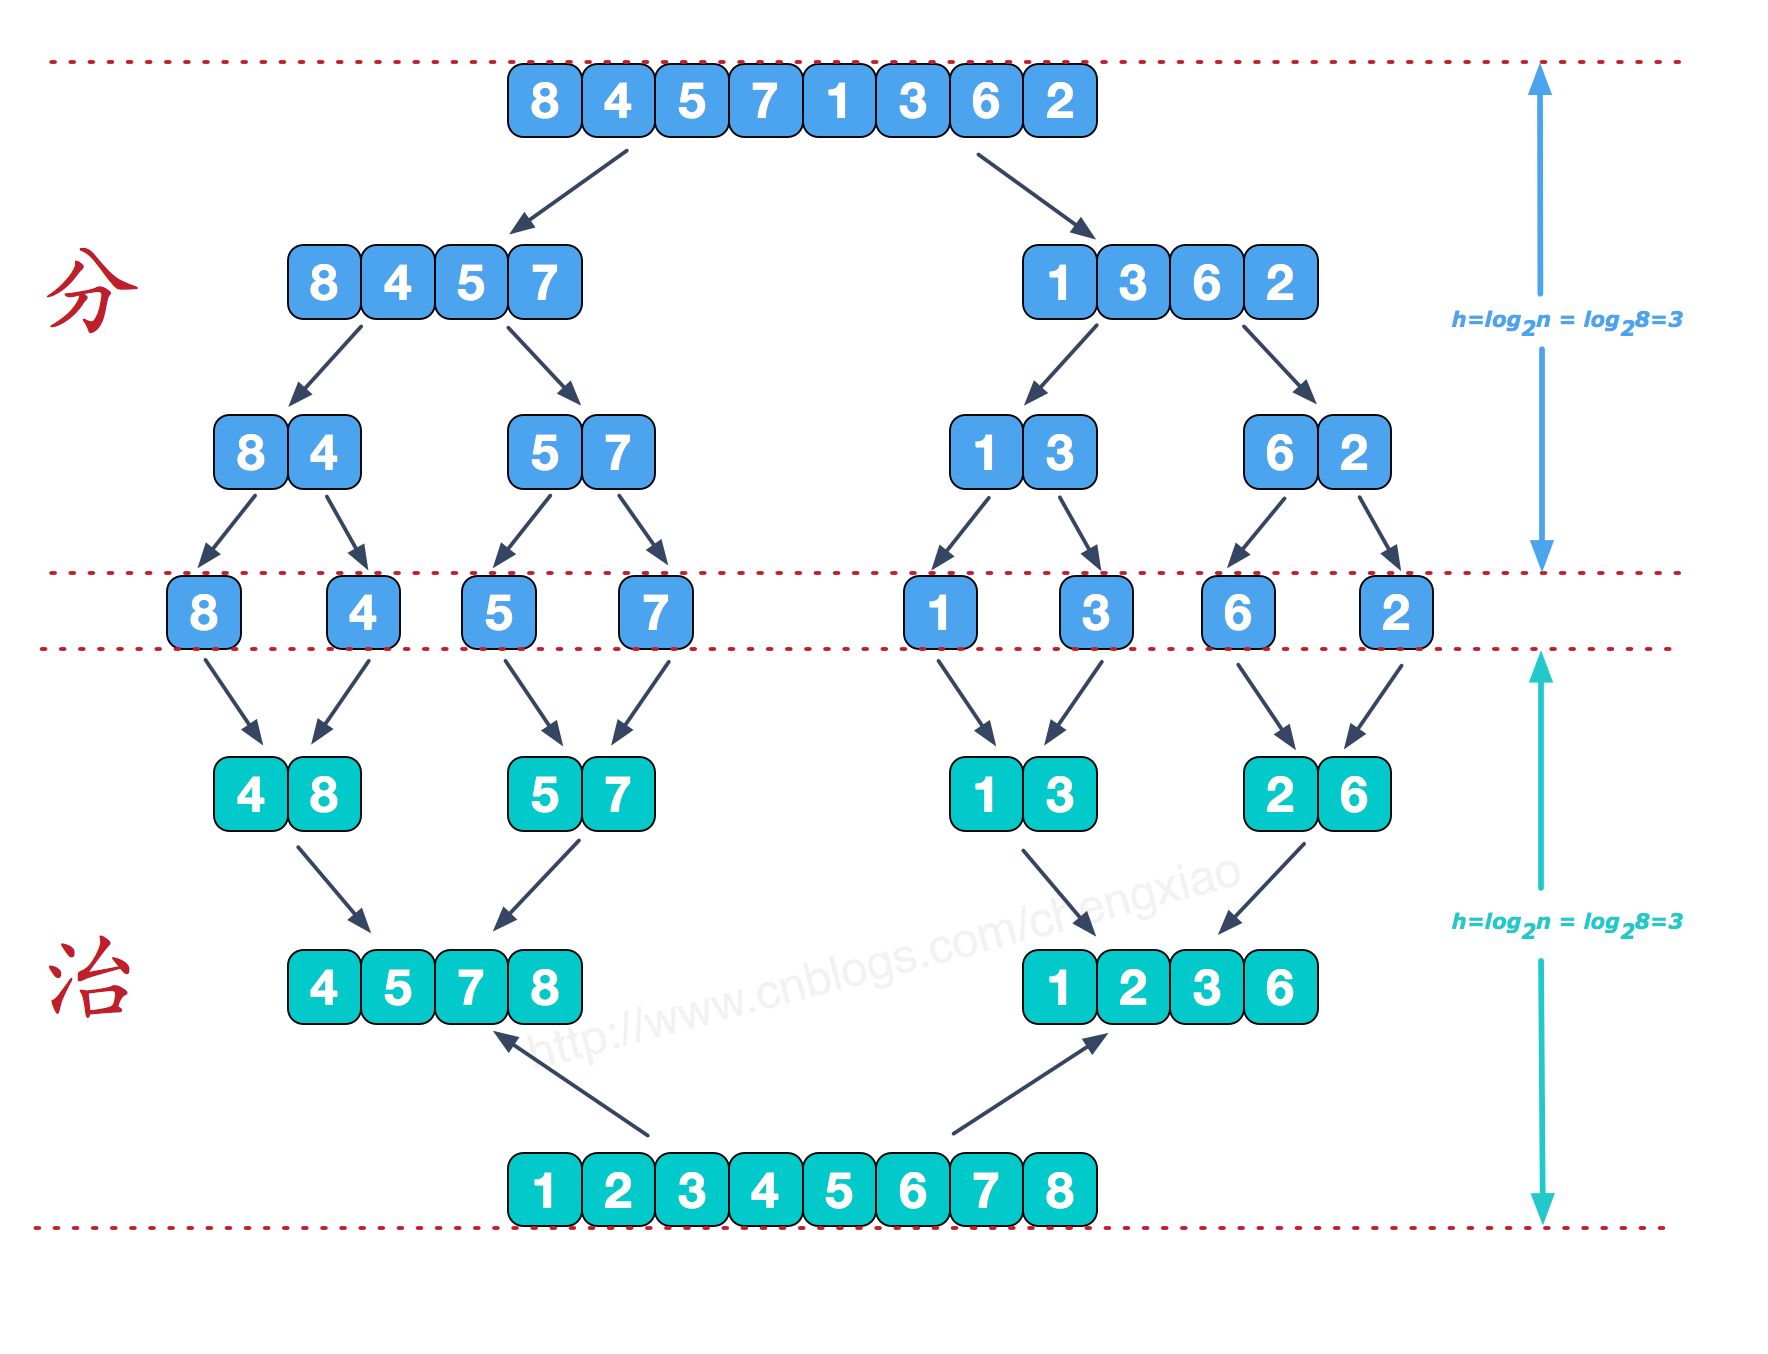
\includegraphics[height=0.7\textheight]{mergesort.png}
\caption{算法示意图(\url{https://www.cnblogs.com/chengxiao/p/6194356.html})}
\end{figure}
\end{frame}

\begin{frame}[fragile]{归并排序}

需要利用的几个工具与知识点:
\begin{itemize}
\item 常用的\texinl|set|赋值函数仅影响组内的值,把函数体封装在组内可以使每一层的函数拥有自己独立的局部变量(类似于其它编程语言中的栈)
\item \texinl|\tl_head:n| 返回凭据表的头一个元素
\item \texinl|\tl_tail:n| 返回凭据表的尾部元素(去除第一个元素)
\item \texinl|\tl_range:nnn| 返回凭据表的一个区间内的所有元素
\item \LaTeX 中的递归函数一般无法直接返回值,我们可以把要返回的值存在一个全局变量中
\end{itemize}

\end{frame}


\begin{frame}[fragile]{归并排序}

\begin{texcode*}
\ExplSyntaxOn
\tl_new:N \g_merge_result_tl
\cs_gset:Npn \my_merge:nn #1#2 {
    \group_begin:
        \bool_set_true:N \l_tmpa_bool
        \tl_if_empty:nT {#1} { \bool_set_false:N \l_tmpa_bool 
            \tl_gput_right:Nn \g_merge_result_tl {#2} }
        \tl_if_empty:nT {#2} { \bool_set_false:N \l_tmpa_bool 
            \tl_gput_right:Nn \g_merge_result_tl {#1} }
        \bool_if:NT \l_tmpa_bool {
            \int_compare:nNnTF {\tl_head:n {#1}} < {\tl_head:n {#2}} 
                { \tl_gput_right:Nx \g_merge_result_tl {{\tl_head:n {#1}}}
                \exp_args:Nx \my_merge:nn {\tl_tail:n {#1}} {#2} } 
                { \tl_gput_right:Nx \g_merge_result_tl {{\tl_head:n {#2}}}
                \exp_args:Nnx \my_merge:nn {#1} {\tl_tail:n {#2}} }
        }
    \group_end:
}
\ExplSyntaxOff
\end{texcode*}

\end{frame}


\begin{frame}[fragile]{归并排序}

\begin{texcode*}
\ExplSyntaxOn
\tl_new:N \g_merge_sort_result_tl
\cs_gset:Npn \my_merge_sort:n #1 {
    \iow_term:n {#1}
    \group_begin:
        \int_compare:nNnTF {\tl_count:n {#1}} > {1} {
            \int_set:Nn \l_tmpa_int {\int_div_truncate:nn {\tl_count:n {#1}}{2}}
            \exp_args:Nx \my_merge_sort:n { \tl_range:nnn {#1} {1} {\l_tmpa_int} }
            \tl_set_eq:NN \l_tmpa_tl \g_merge_sort_result_tl
            \exp_args:Nx \my_merge_sort:n { \tl_range:nnn {#1} {\l_tmpa_int + 1} {\tl_count:n {#1}} } 
            \tl_clear:N \g_merge_result_tl
            \exp_args:NVV \my_merge:nn \l_tmpa_tl \g_merge_sort_result_tl
            \tl_gset_eq:NN \g_merge_sort_result_tl \g_merge_result_tl
        } { \tl_gset:Nn \g_merge_sort_result_tl {#1} }
    \group_end:
}
\ExplSyntaxOff
\end{texcode*}

\end{frame}

\begin{frame}[fragile]{归并排序}

\begin{texcode*}
\ExplSyntaxOn
\my_merge_sort:n {{1}{3}{5}{2}{4}{6}}
\par\cs_meaning:N \g_merge_sort_result_tl
\my_merge_sort:n {{1}{2}{1}{2}{1}{2}}
\par\cs_meaning:N \g_merge_sort_result_tl
\my_merge_sort:n {{9}{8}{7}{6}{5}{4}{3}{2}{1}}
\par\cs_meaning:N \g_merge_sort_result_tl
\my_merge_sort:n {{1}}
\par\cs_meaning:N \g_merge_sort_result_tl
\ExplSyntaxOff
\end{texcode*}


\end{frame}

\end{document}